% !TEX root = ../../../main.tex
% 来源：中学数学实验教材·第三册（高中数学）
% 章节：函数及其图象 / 函数及其图象
% 原始文件：4.tex，行 795-805
% 类型：tikz
% ---
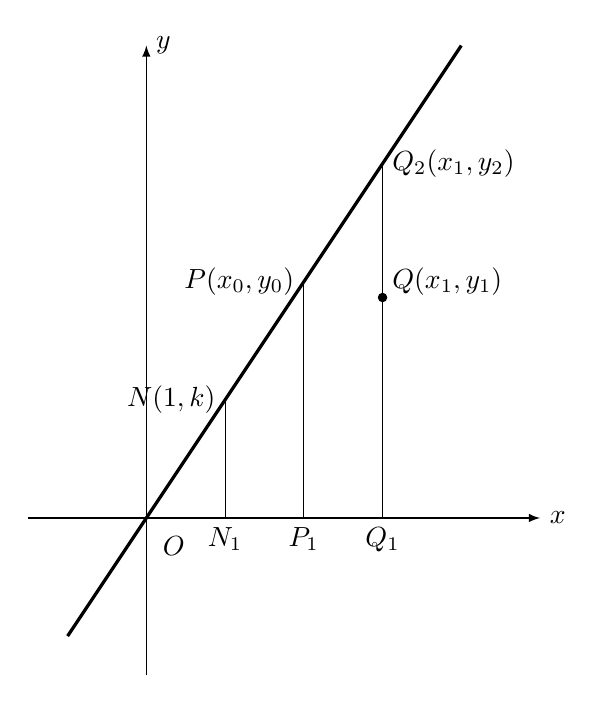
\begin{tikzpicture}[>=latex]
    \draw[->](-1.5,0)--(5,0)node[right]{$x$};
    \draw[->] (0,-2)--(0,6)node[right]{$y$};
\node at (.35,-.35){$O$};
\draw[very thick] (-1,-1.5)--(4,6);    
\draw (1,0)node[below]{$N_1$}--(1,1.5)node[left]{$N(1,k)$};
\draw (2,0)node[below]{$P_1$}--(2,3)node[left]{$P(x_0,y_0)$};
\draw (3,0)node[below]{$Q_1$}--(3,4.5)node[right]{$Q_2(x_1,y_2)$};
\node at (3,3)[right]{$Q(x_1,y_1)$};
\draw (3,2.8)[fill=black] circle (1.5pt);
\end{tikzpicture}
